%%%%%%%%%%%%%%%%%%%%%%%%%%%%%%%%%%%%%%%%%
% Beamer Presentation
% LaTeX Template
% Version 1.0 (10/11/12)
%
% This template has been downloaded from:
% http://www.LaTeXTemplates.com
%
% License:
% CC BY-NC-SA 3.0 (http://creativecommons.org/licenses/by-nc-sa/3.0/)
%
%%%%%%%%%%%%%%%%%%%%%%%%%%%%%%%%%%%%%%%%%

%----------------------------------------------------------------------------------------
%	PACKAGES AND THEMES
%----------------------------------------------------------------------------------------

\documentclass{beamer}

\mode<presentation> {

% The Beamer class comes with a number of default slide themes
% which change the colors and layouts of slides. Below this is a list
% of all the themes, uncomment each in turn to see what they look like.

%\usetheme{default}
%\usetheme{AnnArbor}
%\usetheme{Antibes}
%\usetheme{Bergen}
\usetheme{Berkeley}
%\usetheme{Berlin}
%\usetheme{Boadilla}
%\usetheme{CambridgeUS}
%\usetheme{Copenhagen}
%\usetheme{Darmstadt}
%\usetheme{Dresden}
%\usetheme{Frankfurt}
%\usetheme{Goettingen}
%\usetheme{Hannover}
%\usetheme{Ilmenau}
%\usetheme{JuanLesPins}
%\usetheme{Luebeck}
%\usetheme{Madrid}
%\usetheme{Malmoe}
%\usetheme{Marburg}
%\usetheme{Montpellier}
%\usetheme{PaloAlto}
%\usetheme{Pittsburgh}
%\usetheme{Rochester}
%\usetheme{Singapore}
%\usetheme{Szeged}
%\usetheme{Warsaw}

% As well as themes, the Beamer class has a number of color themes
% for any slide theme. Uncomment each of these in turn to see how it
% changes the colors of your current slide theme.

%\usecolortheme{albatross}
%\usecolortheme{beaver}
%\usecolortheme{beetle}
%\usecolortheme{crane}
%\usecolortheme{dolphin}
%\usecolortheme{dove}
%\usecolortheme{fly}
%\usecolortheme{lily}
%\usecolortheme{orchid}
%\usecolortheme{rose}
%\usecolortheme{seagull}
%\usecolortheme{seahorse}
%\usecolortheme{whale}
%\usecolortheme{wolverine}

%\setbeamertemplate{footline} % To remove the footer line in all slides uncomment this line
%\setbeamertemplate{footline}[page number] % To replace the footer line in all slides with a simple slide count uncomment this line

%\setbeamertemplate{navigation symbols}{} % To remove the navigation symbols from the bottom of all slides uncomment this line
}
\usepackage{setspace}
\usepackage{graphicx} % Allows including images
\usepackage{booktabs} % Allows the use of \toprule, \midrule and \bottomrule in tables
%----------------------------------------------------------------------------------------
%	TITLE PAGE
%----------------------------------------------------------------------------------------

\title[]{Loop Acceleration For Tightly-Coupled CPU+FPGA System} 
\author[]{
    Cheng Liu 
    \\Supervisor: Dr. Hayden Kwok-Hay So 
    \\Co-supervisor: Dr. Ngai Wong}
\institute {
    Department of Electrical and Electronic Engineering 
    \\The University of Hong Kong
\medskip
}
\date{\today} % Date, can be changed to a custom date

\graphicspath{{./figures/}} 
\begin{document}

\begin{frame}
\titlepage % Print the title page as the first slide
\end{frame}

%----------------------------------------------------------------------------------------
%	PRESENTATION SLIDES
%----------------------------------------------------------------------------------------

%------------------------------------------------
\section{Background} 
%------------------------------------------------
\begin{frame}[t]
\frametitle{FPGA vs. CPU vs. GPU}
\textbf{FPGA has competitive computation capability and \\
        energy efficiency.} 

\begin{figure}
  \vspace{-1em}
  \includegraphics[width=.8\linewidth]{performance-cpu-fpga-gpu}
  \vspace{-1em}
\end{figure}
\begin{figure}
  \vspace{-1em}
  \includegraphics[width=.8\linewidth]{energy-cpu-fpga-gpu}
  \vspace{-1em}
\end{figure}

\begin{spacing}{1.2}
\tiny{[1] Eric S. Chung, etc., Single-Chip Heterogeneous Computing: Does the future include customized
logic, FPGA and GPGPUs?, IEEE International Symposium of Microarchitecture, 2010}
\end{spacing}

\end{frame}

%------------------------------------------------
\begin{frame}[t]

\frametitle{Why isn't FPGA the mainstream computing device?}
\textbf{Main obstacles}
\begin{itemize}

\item High barrier-to-entry
\begin{itemize}
\item Require hardware knowledge for both design and debug.
\item More software engineers than hardware engineers.
\item ...
\end{itemize}

\item Low design productivity
\begin{itemize}
\item Low level abstraction and long development time
\item Long compilation and implementation time
\item Poor portability and design reuse
\item Unable to support complex software like OS
\item ...
\end{itemize}

\end{itemize}

\end{frame}

%------------------------------------------------
\begin{frame}[t]
\frametitle{What has the community done to overcome the obstacles?}

\textbf{Design methodologies}
\begin{itemize}
\item High level synthesis languages and tools \\
\footnotesize
Vivado(Xpilot, AutoESL), LegUP, Impulse-C, ...
\normalsize

\item Communication libraries, unified memory interfaces, and integrated environments \\
\footnotesize
CoRAM, LEAP, ...
\normalsize

\item Virtual overlay on top of commerical FPGA \\
\footnotesize 
VirtualRC, Soft coarse-grained reconfigurale array (SCGRA), ...
\normalsize

\end{itemize}

\textbf{Computation architectures}
\begin{itemize}
\item Hybrid computation architectures \\
\footnotesize
Embedded softcore+FPGA, Embedded hardcore+FPGA, General CPU+FPGA, ...
\normalsize
\end{itemize}

\end{frame}

%------------------------------------------------
\begin{frame}[t]
\frametitle{Differences and relations of the design methodologies}

\begin{figure}
  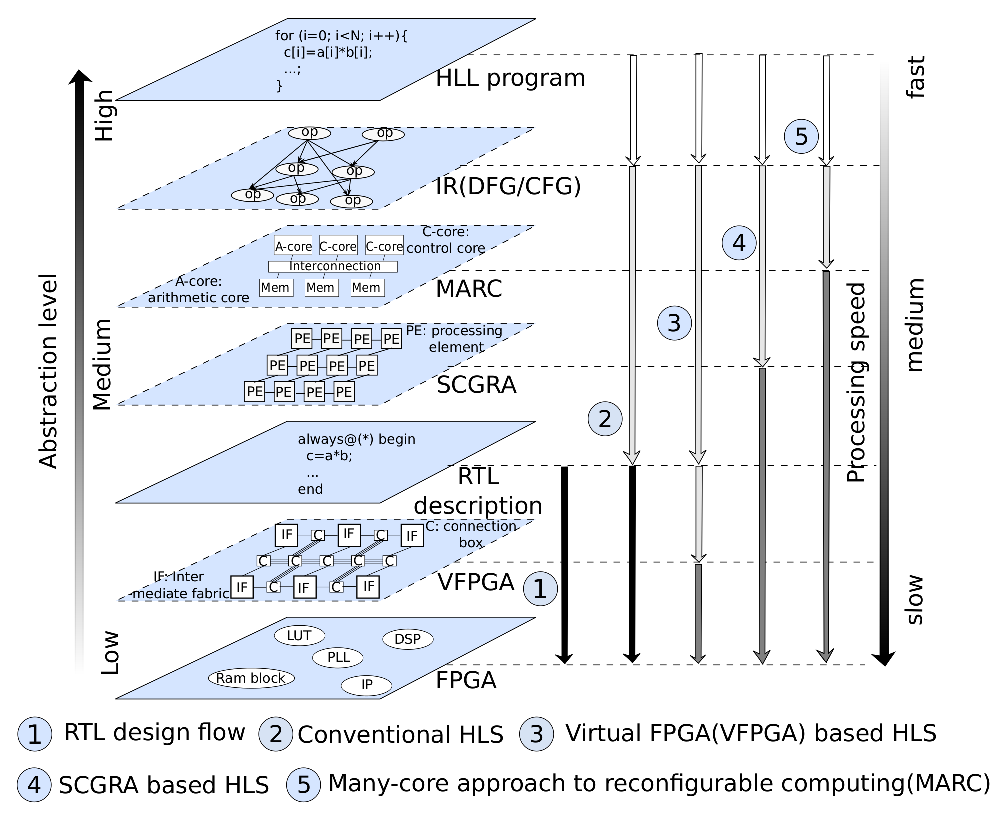
\includegraphics[width=.8\linewidth]{virtual-overlay}
\end{figure}

\end{frame}

%------------------------------------------------
\begin{frame}[t]

\frametitle{Trade-offs under the hood?}
\textbf{Performance vs. productivity/flexibility}

\end{frame}

%------------------------------------------------
\begin{frame}[t]
\frametitle{CPU+FPGA accelerator}
\textbf{Computation kernel}
\begin{itemize}
\item Sequential programming model.
\item Loop is typical computation kernel.
\end{itemize}

\textbf{CPU+FPGA accelerator}
Include CPU+FPGA accelerator as well as the compiling flow

\end{frame}

%------------------------------------------------
\begin{frame}[t]
\frametitle{Trade-offs with the CPU+FPGA accelerator}
\begin{itemize}
\item High barrier-to-entry (Hardware engineering skills, ...)
\item Low design productivity (Low level abstraction, Long compilation time, ...)
\item Complex design space exploration
\item ...
\end{itemize}
\end{frame}


%------------------------------------------------
\section{Related work}
%------------------------------------------------
\begin{frame}
\frametitle{Contemporary FPGA accelerator design methods}
\textbf{Classification through design entry}
\begin{itemize}
\item Register transfer level (RTL) design flow
\item High level synthesis based design flow
\end{itemize}

\textbf{Classification through compilation}
\begin{itemize}
\item Compile to HDL and implementation on FPGA
\item Comple to virtual overlay, implementation on overlay and implementation on FPGA
\end{itemize}

\end{frame}

%------------------------------------------------
\begin{frame}

\frametitle{Comparison of different design methods}
Performance and productivity.

\end{frame}

%------------------------------------------------
\begin{frame}

\frametitle{Limitation of previous SCGRA work}
\begin{itemize}
\item Ignore the loop structure
\item Ignore the communication limitation
\end{itemize}

\end{frame}

%------------------------------------------------
\section{Research scheme}
\begin{frame}

\frametitle{System overview}
SCGRA based CPU+FPGA accelerator.

\end{frame}

%------------------------------------------------
\begin{frame}
\frametitle{Design space overview}
Complex design space

\end{frame}

%------------------------------------------------
\begin{frame}

\frametitle{Research focuses}
\begin{itemize}
\item Loop unrolling
\item Operation scheduling
\item Communication interface
\end{itemize}

\end{frame}

%------------------------------------------------
\begin{frame}

\frametitle{Automatic loop optimization}
\begin{itemize}
\item Loop unrolling analysis
\end{itemize}

\end{frame}

%------------------------------------------------
\begin{frame}

\frametitle{Operation scheduling}
\begin{itemize}
\item IO aware
\item On chip memory aware
\item memory footprint aware
\end{itemize}

\end{frame}

%------------------------------------------------
\begin{frame}

\frametitle{Communication interface}
\begin{itemize}
\item Data prefetching
\item On chip buffer synthesis
\end{itemize}

\end{frame}



%------------------------------------------------
\section{Current progress}
\begin{frame}

\frametitle{Design productivity oriented design flow}
Design flow developed to improvde design productivity.

\end{frame}

%------------------------------------------------
\begin{frame}

\frametitle{Preliminary loop unrolling analysis}
%\footnotesize{
%\begin{thebibliography}{99} % Beamer does not support BibTeX so references must be inserted manually as below
%\bibitem[Smith, 2012]{p1} John Smith (2012)
%\newblock Title of the publication
%\newblock \emph{Journal Name} 12(3), 45 -- 678.
%\end{thebibliography}
%}
\end{frame}

%------------------------------------------------
\begin{frame}

\frametitle{HW/SW communication on Zedboard}
HW/SW communication on Zedboard

\end{frame}

%------------------------------------------------
\section{Conclusion}
\begin{frame}
\Huge{\centerline{The End}}
\end{frame}

%------------------------------------------------

\end{document} 
